\documentclass[11pt]{article}
\usepackage{geometry}
\usepackage{graphicx}
\usepackage{hyperref}
\usepackage{listings}
\usepackage{xcolor}
\usepackage{tcolorbox}
\usepackage{float}

\geometry{a4paper, margin=1in}

\title{\textbf{CY-Truck Project: Advanced Data Analysis System for Logistics Management}}
\author{N.Guihot \\ E.Szpoper \\ N.Rayée }
\date{}

\tcbuselibrary{listings,skins}

\lstdefinestyle{mystyle}{
    backgroundcolor=\color{white},
    commentstyle=\color{white},
    keywordstyle=\color{white},
    numberstyle=\tiny\color{white},
    stringstyle=\color{white},
    basicstyle=\color{white},
    breakatwhitespace=false,
    breaklines=true,
    captionpos=b,
    keepspaces=true,
    numbers=left,
    numbersep=5pt,
    showspaces=false,
    showstringspaces=false,
    showtabs=false,
    tabsize=2,
}

\lstset{style=mystyle}

\newtcolorbox{mycode}[1][]{
    boxrule=0pt,
    boxsep=0pt,
    arc=4pt,
    outer arc=4pt,
    left=5pt,
    right=5pt,
    bottom=5pt,
    top=5pt,
    listing only,
    listing options={style=mystyle},
    before=\par\smallskip\noindent, % Add a small space before the box and prevent indentation
    after=\par\smallskip, % Add a small space after the box
    #1
}

\begin{document}

\maketitle

\begin{figure}
    \centering
    
\includegraphics[scale=0.5]{cyl.png}
\end{figure}


\tableofcontents
\newpage
\begin{center}
    
\includegraphics[scale=0.2]{logo.png} \\
    Coding the Future of Transport
\end{center}


\section{Introduction}
The \textbf{\color{blue}CY-Truck}  project is designed to revolutionize data processing in logistics. The team includes N. Guihot, E. Szpoper, and N. Rayée, each with distinct roles contributing to the project's success.

\subsection{About the project}
The CY Truck project, led by Eva Ansermin and Romuald Grignon, involves creating a program to manage the logistics of a national road transport company. This project addresses the challenge of manually processing large and varied logistics data. The program is designed to analyze a data file and generate graphs summarizing the company's activities.

\subsubsection{Development of a Shell Script and a C Program}
The Shell script, along with a C program for performance operations, analyzes the data file and creates graphs.

\subsubsection{Data Management and Processing}
The program manages a CSV file containing road trip data, including 'RouteID', 'StepID', 'Departures', 'Arrivals', 'Distance', and 'DriverNames'.

\subsubsection{Graph Creation using GnuPlot}
After processing the data, the Shell script uses GnuPlot to create graphs illustrating various aspects of the data, such as drivers with the most trips, longest distances traveled, longest trips, and most traversed cities.

\subsubsection{Organization and Storage of Data and Results}
Input data, programs, graphs, and intermediate files are organized into specific folders for better management.

\subsubsection{Flexibility and Scalability}
The project is designed to be scalable, with options for enhancement and adaptation to specific needs.

\newpage
\section{Getting Started}

This project requires several tools and packages to be installed on your system. Ensure you have the following prerequisites installed before proceeding with the project setup.

\subsection{Prerequisites}

\begin{itemize}
    \item GnuPlot is used for generating graphs from data. Install it via your system's package manager. For example, on Ubuntu:
          \begin{mycode}
              sudo apt-get install gnuplot
          \end{mycode}

    \item Make is a build automation tool that automatically builds executable programs and libraries. Install it as follows:
          \begin{mycode}
              sudo apt-get install make
          \end{mycode}

    \item ImageMagick is a software suite to create, edit, compose, or convert bitmap images. It can be installed with:
          \begin{mycode}
              sudo apt-get install imagemagick
          \end{mycode}
\end{itemize}
Ensure that all these tools are correctly installed on your system. They are essential for running and managing various aspects of the project, from data processing to image manipulation.

\subsection{Installation}

\begin{itemize}
    \item Clone the repo
          \begin{mycode}
              git clone https://github.com/guinat/Projet\_CY\_Truck\_preIng2\_2023\_2024.git
          \end{mycode}


    \item After performing a git clone of the repository, navigate to the project directory with the following command:
          \begin{mycode}
              cd Projet\_CY\_Truck\_preIng2\_2023\_2024
          \end{mycode}
\end{itemize}

\section{Usage}
This section guides you through the steps to execute and use the CY Truck program. The program is executed via a Shell script that processes a CSV file and generates various outputs based on the options provided.

\subsection{Preparing the Data File}
Ensure that you have the CSV file containing the road trip data prepared and ready for use. This file should include the following details, listed in order: 'RouteID', 'StepID', 'Departures', 'Arrivals', 'Distance', and 'Driver Names'.

\subsection{Running the Script}
\begin{itemize}
    \item Before running the script, ensure that your main script has the necessary permissions to be executed. You can grant execute permission using the following command in your terminal
          \begin{mycode}
              chmod +x main.sh
          \end{mycode}

    \item To execute the program, use the following command format in your terminal. Replace [path\_to\_csv\_file] with the actual path to your CSV file and [option] with the desired operation option.
          \begin{mycode}
              ./main.sh [path\_to\_csv\_file] [option]
          \end{mycode}
\end{itemize}

\newpage
\subsection{Understanding the Options}
The \textbf{\color{blue}[option]} in the command represents various operations you can perform with the script. Here is the list of available options:


\subsubsection*{Option: \color{blue}-h}
This option displays a help message explaining the available options for the script. It's useful for users who need guidance on how to use the script and what parameters to input.

\subsubsection*{Option: \color{blue}-d1}

This option is for processing and generating a horizontal histogram graph showing the top 10 drivers with the most trips. It sorts the drivers by the number of trips they have made in descending order and displays this information graphically.

\vspace*{\fill}
\begin{center}
    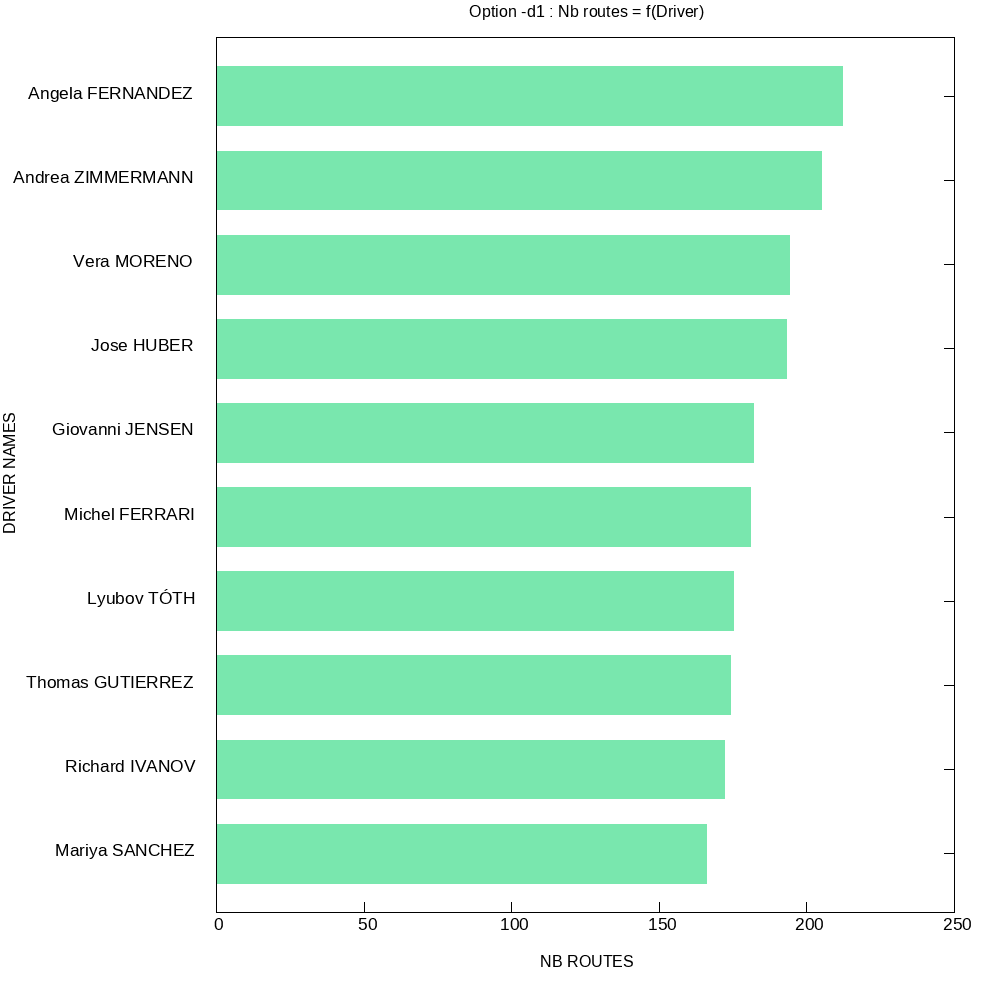
\includegraphics[width=\textwidth]{d1_graph.png}
\end{center}
\vspace*{\fill}

\newpage
\subsubsection*{Option: \color{blue}-d2}
When using this option, the script calculates the total distance traveled by each driver and generates a horizontal histogram graph. It focuses on the top 10 drivers who have covered the longest distances, sorted in descending order of distance traveled.

\vspace*{\fill}
\begin{center}
    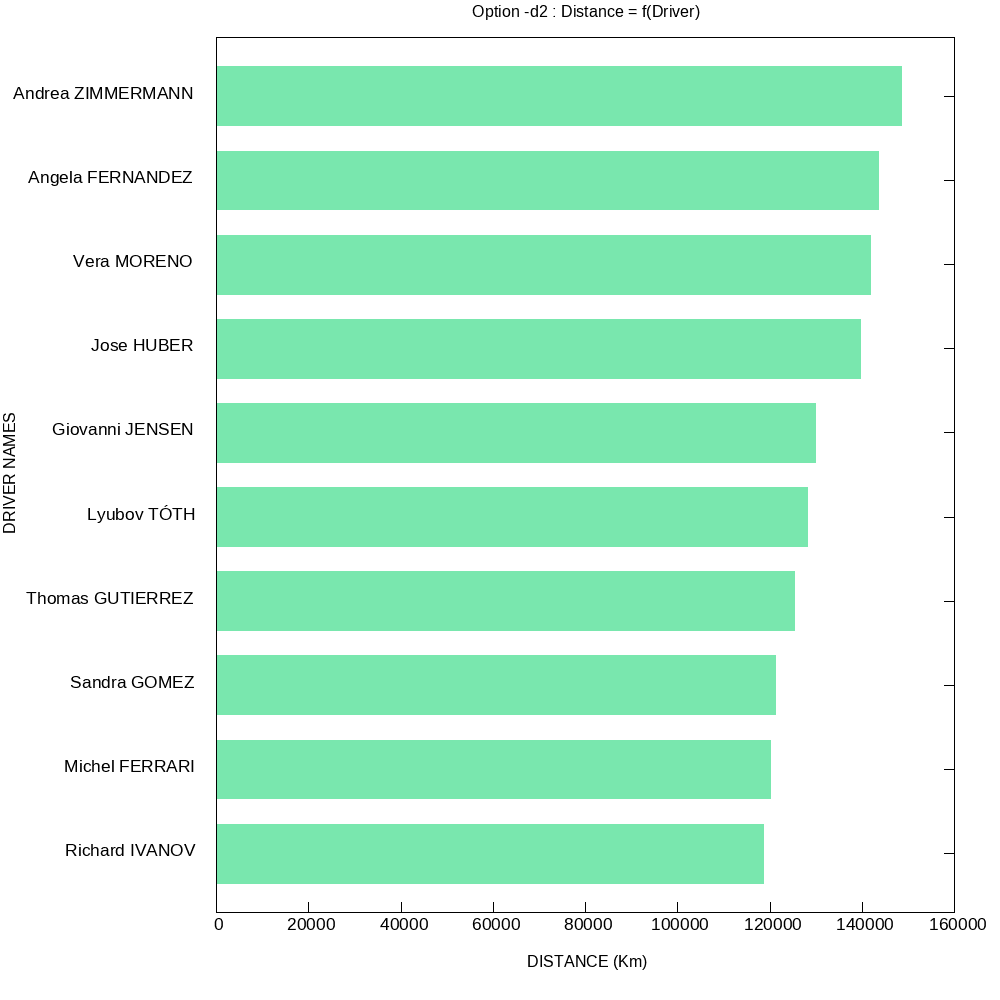
\includegraphics[width=\textwidth]{d2_graph.png}
\end{center}
\vspace*{\fill}

\newpage
\subsubsection*{Option: \color{blue}-l}
This option identifies the 10 longest trips based on total distance. It processes the data to sum up the distance for each trip and then generates a vertical histogram graph, sorting the results by trip identifier in ascending order.

\vspace*{\fill}
\begin{center}
    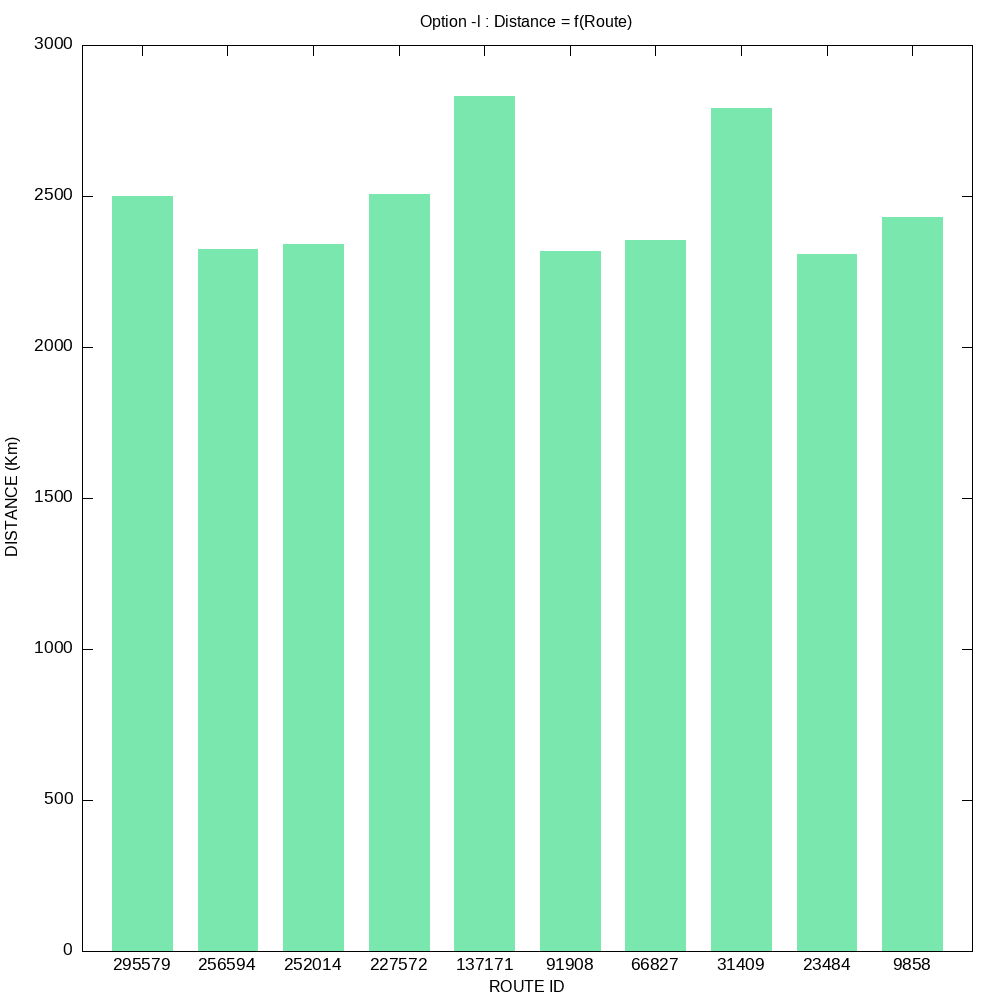
\includegraphics[width=\textwidth]{l_graph.png}
\end{center}
\vspace*{\fill}

\newpage
\subsubsection*{Option: \color{blue}-t}
When selected, this option counts the number of trips passing through each city and the number of times these cities are starting points of trips. It then creates a grouped histogram graph for the top 10 cities, sorted alphabetically, showing the total number of trips through each city and the number of times they are trip starting points.

\vspace*{\fill}
\begin{center}
    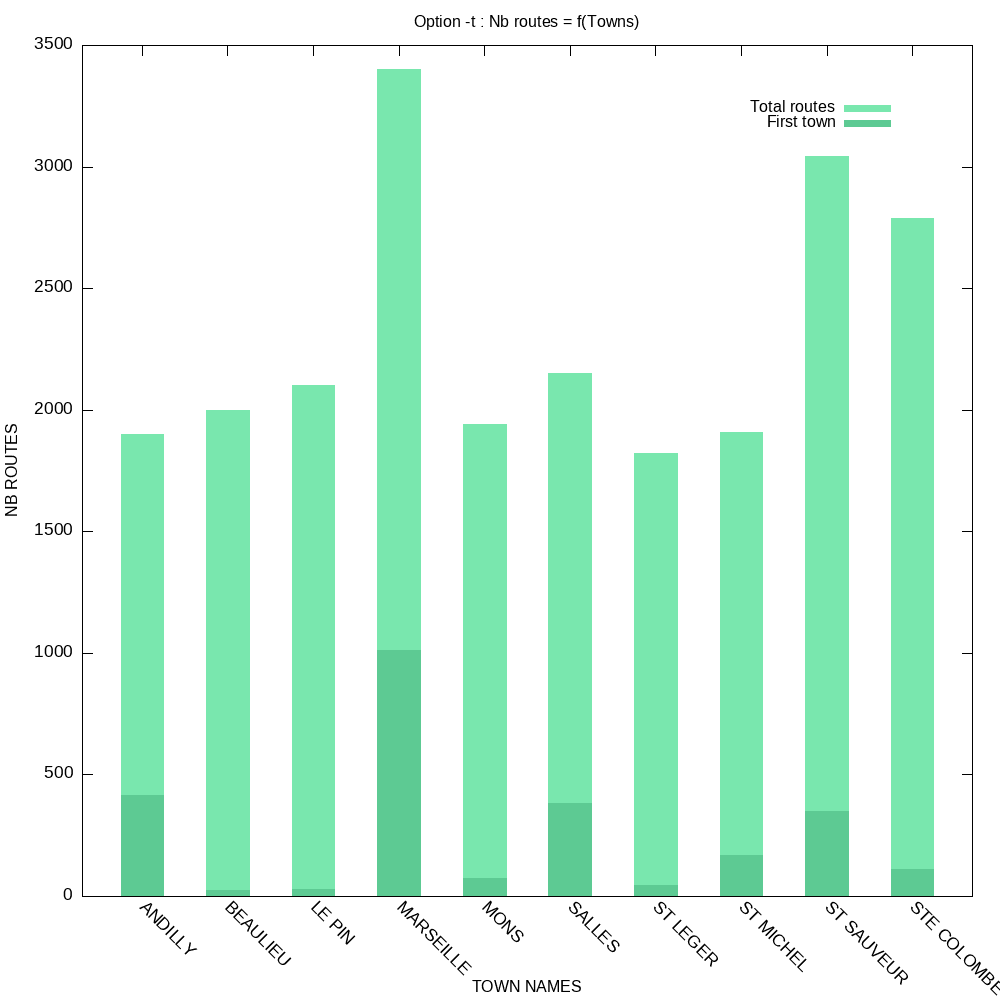
\includegraphics[width=\textwidth]{t_graph.png}
\end{center}
\vspace*{\fill}

\newpage
\subsubsection*{Option: \color{blue}-s}
This option is designed to gather statistics on the stages of each trip, such as minimum, maximum, and average distances. It creates a min-max-average curve graph, displaying these values for the top 50 trips, sorted by the difference between maximum and minimum distances in descending order.

\vspace*{\fill}
\begin{center}
    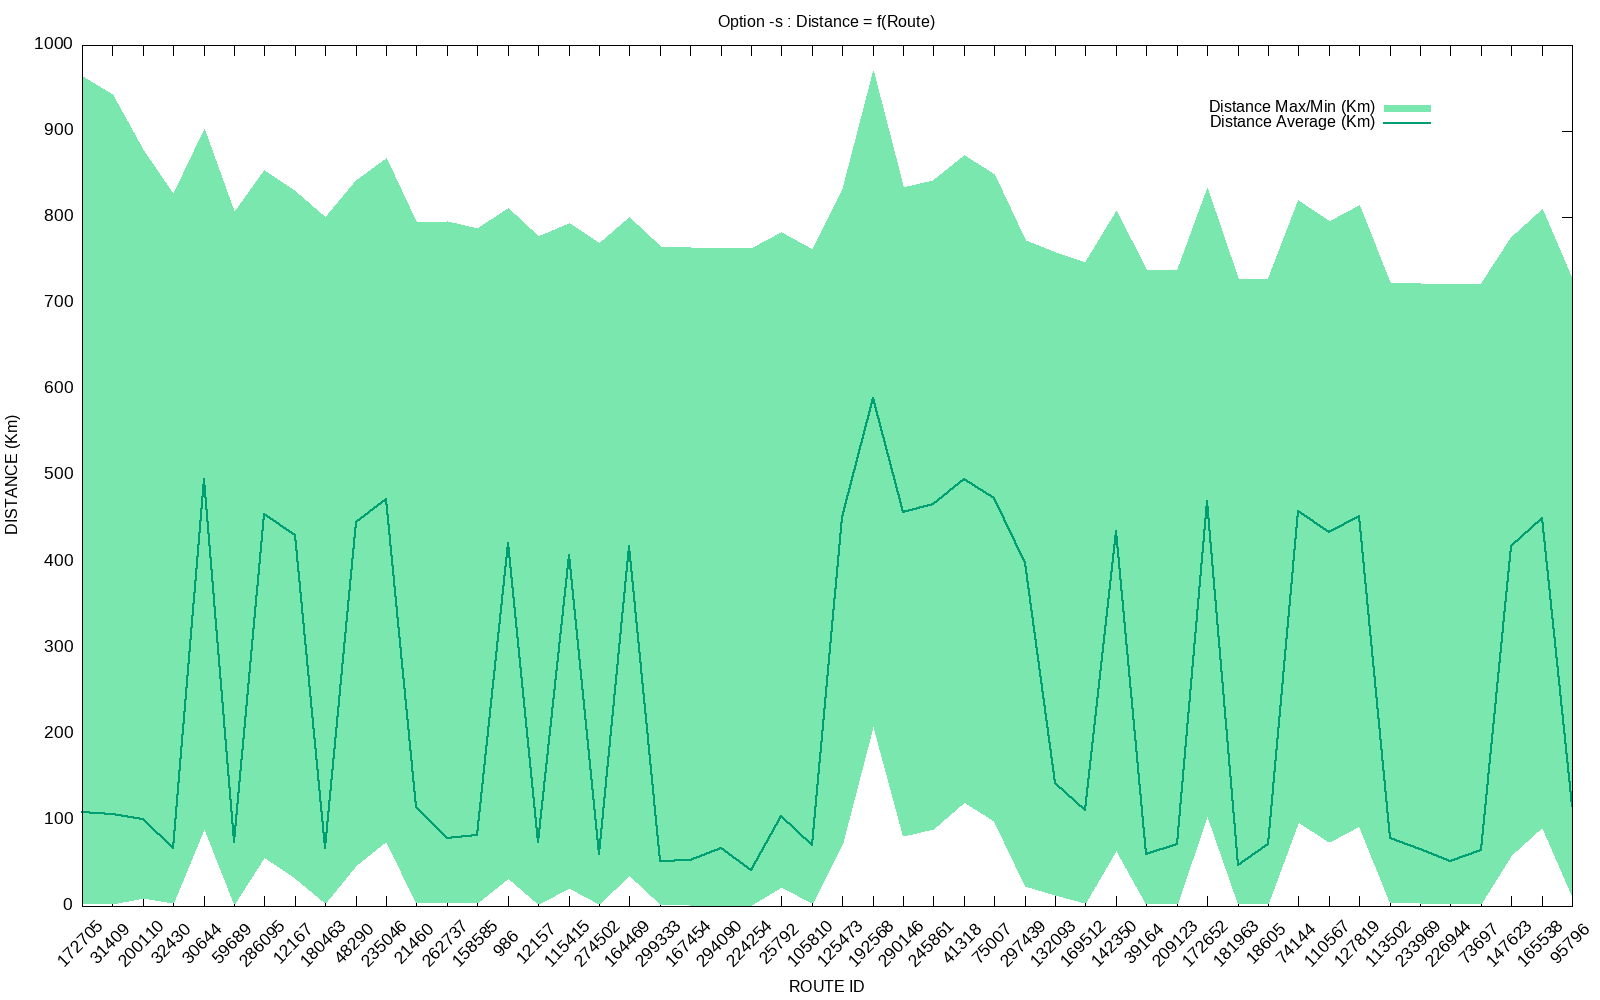
\includegraphics[width=\textwidth]{s_graph.png}
\end{center}
\vspace*{\fill}



\newpage
\section{Task Allocation}
\subsection{N. Guihot - Project Structuring and C Programming}
\begin{itemize}
    \item \textbf{Resource Provision}: Identifying and providing essential tools and resources.
    \item \textbf{Task Distribution}: Assigning tasks based on skills and ensuring a balanced workload.
    \item \textbf{Performance Optimization}: Enhancing the efficiency of the C program in execution and memory usage.
    \item \textbf{Data Processing for T and S}: Implementing and optimizing data processing for project parts T and S.
    \item \textbf{Version Management and Documentation}: Setting up version control using Git and creating technical documentation.
    \item \textbf{Data Security}: Implementing secure practices for data handling and storage.
    \item \textbf{Project Report Writing}: Preparing a detailed project report on task distribution, project timeline, and application limitations.
\end{itemize}

\subsection{E. Szpoper - Main Script Management}
\begin{itemize}
    \item \textbf{Data Processing for D1 and D2}: Implementing and optimizing data processing for project parts D1 and D2.
    \item \textbf{Script Component Functionality Assurance}: Ensuring effective operation of all script components.
    \item \textbf{Team Meeting Planning and Organization}: Scheduling regular meetings for project updates and planning.
    \item \textbf{Shared Resource Management}: Managing access to shared resources like documents and software tools.
    \item \textbf{Test Automation}: Developing scripts for automated testing of script components.
    \item \textbf{Robustness Testing}: Ensuring the program handles errors and unexpected data inputs effectively.
\end{itemize}

\subsection{N. Rayée - GnuPlot and Graphical Generation}
\begin{itemize}
    \item \textbf{Graph Creation for Each Treatment}: Designing and generating graphs for each data treatment.
    \item \textbf{Data Visualization Using Temporary Data Files}: Creating visualizations from interim data files.
    \item \textbf{Documentation and Archiving}: Documenting and archiving all materials, including code and reports.
    \item \textbf{Time and Priority Management}: Using project management tools for tracking deadlines and prioritizing tasks.
    \item \textbf{Code Quality Assurance}: Establishing coding standards and conducting code reviews.
    \item \textbf{Code Review Organization}: Organizing sessions to review code for cleanliness, documentation, and best practices.
    \item \textbf{Delivery Planning and Deadlines}: Setting and adhering to a timeline for different project phases.
\end{itemize}

\section{Project Timeline}

\subsection{Project Organization}
Our project followed a rigorous and structured approach, emphasizing daily progress and continuous communication. We committed to making near-daily deposits to our Git repository, ensuring a consistent and trackable development process. Additionally, we held daily calls via Discord or WhatsApp to discuss progress, address immediate issues, and plan for upcoming tasks. This regular rhythm of coding and communication was crucial for maintaining project momentum and aligning team efforts.

\vspace{0.5cm}

\begin{tabular}{|l|p{10cm}|}
    \hline
    Date           & Activity                                                                     \\
    \hline
    Day 1: Dec 19  & Initial project setup - First commit.                                        \\
    Day 2: Dec 20  & Data processing update for D1, performance optimization, and color addition. \\
    Day 3: Dec 21  & Implementation of alert management features.                                 \\
    Day 4: Dec 22  & Enhancement of graph generation for D1.                                      \\
    Day 5: Dec 23  & Implementation of -d1 option.                                                \\
    Day 6: Dec 24  & Addition of new features: options processing, D2, and L treatments.          \\
    Day 7: Dec 25  & Start of -t option development.                                              \\
    Day 9: Dec 27  & Completion of -t option.                                                     \\
    Day 10: Dec 28 & "Almost finished" - Finalizing features.                                     \\
    Day 11: Dec 29 & Final additions and adjustments.                                             \\
    Day 12: Jan 24 & Added a data file verification function.                                     \\
    Day 13: Jan 25 & Updating the pdf (TODO: Modify processing -t)                                \\
    Day 14: Jan 26 & Testing for t\_processing                                                    \\
    Day 15: Jan 27 & Again testing...                                                             \\
    Day 16: Jan 28 & Done with t\_processing                                                      \\
    \hline
\end{tabular}

\section{Functional Limitations}
\subsection{Unimplemented Features}
Following the error in the data.csv input file, we had to pre-filtrate the file with an awk command. Then using an avl, we establish the requested classification.
We tried to do otherwise, we transformed the file into a large AVL. Which each node contains the routeID and all the stages of this route. We can therefore completely sort this file using this AVL.
\subsection{Operational Issues}
While the project has successfully met all the requirements of the specifications as of January 28, 2024, we are continuously working on improving the optimization of treatments D1, D2, and L. These enhancements are focused on increasing efficiency, reducing execution time, and improving memory usage. The current implementation meets the functional requirements, but we aim to achieve even better performance and reliability in these areas.



\section{Conclusion}
This document outlines the CY-Truck project's task distribution, development timeline, and functional limitations, providing a clear view of our project management and technical challenges.

\end{document}
